\documentclass{beamer}
\usepackage{amsmath}
\usepackage{listings}

\let\vec\mathbf
\newcommand{\myvec}[1]{\ensuremath{\begin{pmatrix}#1\end{pmatrix}}}
\providecommand{\sbrak}[1]{\ensuremath{{}\left[#1\right]}}
\providecommand{\brak}[1]{\ensuremath{\left(#1\right)}}
\providecommand{\cbrak}[1]{\ensuremath{\left\{#1\right\}}}

\lstset{
    language=Python,
    frame=single, 
    breaklines=true,
    columns=fullflexible,
    basicstyle=\ttfamily\small,
    keywordstyle=\color{blue},
    stringstyle=\color{purple},
    commentstyle=\color{gray},
    tabsize=4
}

\title{Matrices in Geometry: Q. 8.4.24}
\author{AI24BTECH11031 - Shivram S}
\date{}

\begin{document}
\begin{frame}
    \titlepage
\end{frame}

\begin{frame}
    \tableofcontents
\end{frame}

\section{Problem}
\subsection{Question}
\begin{frame}
    \frametitle{Question}

    The altitude of a right angled triangle is 7 cm less
    than its base. If the hypotenuse is 13 cm, find the
    other two sides.
\end{frame}

\subsection{Variables Used}
\begin{frame}
    \frametitle{Variables Used}

    \begin{table}[h!]
    \centering
    \begin{tabular}[12pt]{ |c| c| c|}
        \hline
        \textbf{Variable} & \textbf{Description} & \textbf{Value}\\
        \hline
        $BC$ & Hypotenuse of the triangle & 13 cm\\
        \hline
        $AB$ & Base of the triangle & $x$ cm\\
        \hline
        $AC$ & Altitude of the triangle & $x - 7$ cm\\
        \hline
    \end{tabular}
    \caption{Variables Used}
    \end{table}
\end{frame}

\section{Solution}
\subsection{Conic Form}
\begin{frame}
    \frametitle{Conic Form}
    Let the length of the base be $x$ cm. The altitude of the triangle is 7 cm less than its base, i.e.,
    $x - 7$ cm. By Pythagoras' Theorem
    \begin{align}
        AB^2 + AC^2 = BC^2 \\
        x^2 + (x - 7)^2 = 13^2 \\
        2x^2 - 14x - 120 = 0 \\
        x^2 - 7x - 60 = 0
    \end{align}
    
    The equation $y = x^2 - 7x - 60$ can be expressed as a conic 
    \begin{align}
        \vec{x}^\top\vec{V}\vec{x} + 2\vec{u}^\top\vec{x} + f = 0 \\
        \vec{V} = \myvec{1 & 0 \\ 0 & 0}, \vec{u} = \myvec{-\frac{7}{2} \\ -\frac{1}{2}}, f = -60
    \end{align}
\end{frame}

\subsection{Intersection with x-axis}
\begin{frame}
    \frametitle{Intersection with $x$-axis}
    
    To find the roots of the equation, we find the points of intersection of the 
    conic with the $x$-axis
    \begin{align}
        \vec{x} = \vec{h} + k\vec{m} \\
        \vec{h} = \myvec{0 \\ 0}, \vec{m} = \myvec{1 \\ 0}
    \end{align}
    The values of $k$ are given by
    \begin{align}
        k_i &= \frac{1}{\vec{m}^\top\vec{V}\vec{m}}\brak{-\vec{m}^\top\brak{\vec{V\vec{h} + \vec{u}}} \pm \sqrt{
            \sbrak{\vec{m}^\top\brak{\vec{V}\vec{h} + \vec{u}}}^2 - g\brak{\vec{h}}\brak{\vec{m}^\top\vec{V}\vec{m}}
        }} \\
        &= \frac{1}{1} \brak{\frac{7}{2} \pm \sqrt{\brak{\frac{7}{2}}^2 + 60}} \\
        k_1 &= -5, k_1 = 12
    \end{align}
\end{frame}


\begin{frame} 
    Hence the points of intersection are
    \begin{align}
        \vec{h} + k\vec{m} = \myvec{-5 \\ 0}, \myvec{12 \\ 0}
    \end{align}

    Hence the solutions of the equation are $x = -5$ and $x = 12$. We reject $x = -5$ as the length of the side
    can't be negative. Hence, the lengths of the sides are
    \begin{align}
        AB = 12\ cm \\
        AC = 7\ cm \\
        BC = 13\ cm
    \end{align}
\end{frame}

\section{Plotting}
\subsection{Figure I}
\begin{frame}
    \frametitle{Figure I}
    \begin{figure}[h!]
        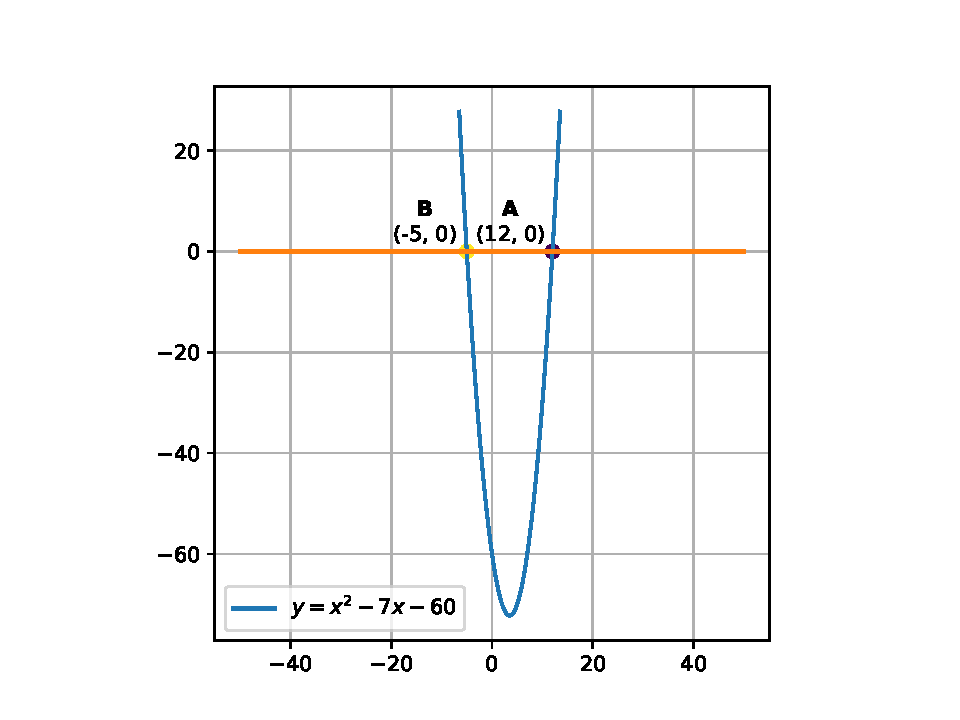
\includegraphics[width=0.9\linewidth]{figs/parabola.pdf}
        \caption{Points of intersection of $y = x^2 - 7x - 60$ with $x$-axis}
    \end{figure}
\end{frame}

\subsection{Python Code I}
\begin{frame}[allowframebreaks]
    \frametitle{Python Code}
    \lstinputlisting{codes/parabola.py}
\end{frame}

\subsection{Figure II}
\begin{frame}
    \frametitle{Figure II}
    \begin{figure}[h!]
        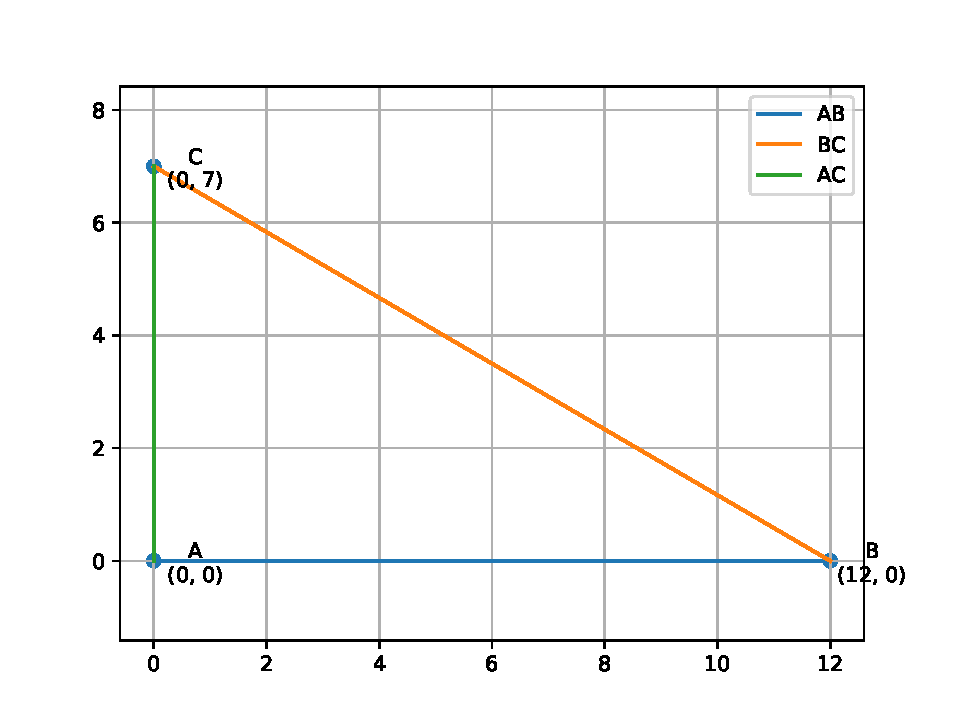
\includegraphics[width=0.9\linewidth]{figs/triangle.pdf}
        \caption{Triangle with sides $AB = 12$ cm, $AC = 7$ cm, and $BC = 13$ cm}
    \end{figure}
\end{frame}

\subsection{Python Code II}
\begin{frame}[allowframebreaks]
    \frametitle{Python Code}
    \lstinputlisting{codes/triangle.py}
\end{frame}

\end{document}